\chapter[Interpolation der Daten "uber Entwaldung]{Interpolation der Daten "uber die Entwaldung des Amazonasgebietes} \label{Kapitel5}
%\minitoc
%\newpage


\section{Die Datengrundlage}
Als Datengrundlage dienen Daten "uber die Entwaldung des Amazonasgebietes die in Form einer SEC"-ONDO-Daten"-bank zur Verf"ugung gestellt wurden. Die Daten aus den Jahren 2004 und 2005 entstanden im Rahmen des DETER-Programms.

\index{DETER}DETER (\textbf{De}tecção de Desmatamento em \textbf{Te}mpo \textbf{R}eal) ist ein Programm der \index{INPE}INPE (\textbf{I}nstituto \textbf{N}acional de \textbf{P}esquisas \textbf{E}spaciais), des brasilianischen Weltraumerforschungszentrums, zur Überwachung des Holzeinschlags am Amazonasgebiet. Der Fokus dieses Programms liegt auf der Erfassung kurzfristiger Veränderungen. \cite{DeF} führt näher aus:
\begin{quotation}
DETER for locations of new deforestation greater than
25 ha in near real-time every two weeks, are based on
a combination of medium and high resolution data using
a mixture model approach to identify changes in
fraction of bare soil and vegetation 
\end{quotation} 
DETER ist nicht unumstritten, \cite{Green} führt aus:
\begin{quotation}
Dieses System erfasst erfahrungsgemäß jedoch nur circa 40 Prozent der zerstörten Fläche.
\end{quotation} 

\newpage
Die DETER--Datenbank besteht aus mehreren Tabellen, die alle den gleichen Aufbau aufweisen. Jede Tabelle steht hierbei für einen Zeitpunkt, zu dem die Flächen aufgenommen wurden. Im Folgenden wird als Beispiel der Tabellenstruktur die Struktur der Tabelle vom 07.05.2004 dargestellt:
\begin{verbatim}
(OBJECT layer20040507 
        ()
        (
            (rel 
                (tuple 
                    (
                        (recordnumber int)
                        (shape region)
                        (layer string)
                        (layerno int))))))
\end{verbatim} 

\begin{figure}
	\centering
	\includegraphics[scale=0.55]{Aufbau_Deter.eps}
	\caption[Inkrementeller Aufbau der Deter--Daten]{Auf dieser Abbildung kann man gut den inkrementiellen Aufbau der Tabellen sehen. Die grünen Flächen entstammen der Aufnahme vom 07.05.2004 und die roten Flächen sind innerhalb von 14 Tagen dazugekommen.\\\textit{\begin{tabular}{ll}
Quelle: &Luftbild, Google Maps;\\
&DETER-Daten dargestellt mit SECONDO
\end{tabular}}}
	\label{fig:Inkrem}
\end{figure}
\newpage
\begin{itemize}
\item recordnumber

ist eine in jedem Layer eindeutige ID.
 
\item shape
 
ist das eigentliche Polygon als Region. Jede Region besteht hier nur aus einem einzigen Face.

\item layer

ist eine textuelle Beschreibung dieser Tabelle und entspricht dem Aufnahmedatum.

\item layerno 

ist eine fortlaufende Nummerierung der einzelnen Tabellen, beginnend mit der Früh"-esten und endend mit der Spätesten.

\end{itemize}
Die einzelnen Layer sind inkrementiell aufgebaut, in dem zweiten Layer sind also nur die Flächen aufgeführt, die seit der letzten Erfassung dazugekommen sind. Dass bei diesem Aufbau Entwaldungsflächen nicht schrumpfen können, ist dem Problem leider angemessen. Abbildung~\vref{fig:Inkrem} veranschaulicht diesen Aufbau.


Die Anzahl der einzelnen Flächen in der Datenbank beträgt insgesamt 30.484, verteilt auf 19 Layer. Auf jeden Layer entfallen also durchschnittlich 1.600 Flächen.
 
Betrachtet wurde der Zeitraum zwischen 07.05.2004 und 30.09.2005.

\section{Die Aufarbeitung der Daten}

Das erste Problem bei der Verarbeitung der Daten ist die zu kleinteilige Erfassung der Polygone der einzelnen Layer. Es gibt in jedem Layer mehrere Polygone, die direkt nebeneinander liegen bzw. sich sogar überlappen. Für eine erfolgreiche Weiterverarbeitung ist eine Zusammenfassung dieser Polygone erforderlich.

Das nächste Problem ist, dass die einzelnen Layer inkrementiell aufgebaut sind, also die Beobachtung zu einem bestimmten Datum aus allen älteren Layern mit dem aktuellen zusammengesetzt werden muss.

In einem ersten Schritt müssen also neue Layer erzeugt werden, so dass gilt:

\begin{enumerate}
\item Ein neues Layer muss die Daten des nächstälteren Layer und Daten des Zieldatums enthalten.
\item In dem neuen Layer müssen alle benachbarten Polygone zu einem Einzigen vereinigt werden.
\end{enumerate}

Am Beispiel des 21.05.2004 werden im Folgenden werden die konkreten Schritte angegeben, um einen neuen Layer zu erzeugen.
\begin{enumerate}
\item  Zuerst müssen die Layer \textbf{layer20040507b} und \textbf{layer20040521} vereinigt werden. Bei dem ersten Layer überhaupt kann dieser Schritt natürlich entfallen. Dies leistet die Anweisung: 

\begin{verbatim}
let tmp = layer20040507b feed layer20040521 feed mergeunion consume
\end{verbatim}
\item Im nächsten Schritt werden alle zusammengehörigen Polygone zusammengefasst.

\begin{verbatim}
let tmp2 = connectedcomponents (
tmp feed {s} tmp feed {t} spatialjoin [shape_s,shape_t] 
constgraph [recordnumber_s,recordnumber_t,fun (i:int) 1.0] ) 
extend [shape: vertices (.Graph) extend [Key:key (.Vertex) ] 
tmp feed 
sortmergejoin [Key,recordnumber] 
aggregateB [shape; fun (r1:region,r2:region) 
union_new (r1,r2); [const region value()] ] ] 
project [shape] consume
\end{verbatim}
Der \textit{spatialjoin} von \textbf{tmp} mit sich selbst liefert alle Paare von zusammengehörigen Polygonen, die dann als Kanten in einem Graphen eingetragen werden, der mittels \textit{constgraph} erzeugt wird. Die Zusammenhangskomponenten dieses Graphen sind nun die zusammengehörigen Polygone. Jede Zusammenhangskomponente wird mit \textit{vertices} in seine Ecken zerlegt, die mit \textit{key} in einen Strom von ID's zerlegt werden. Dieser Strom wird mittels \textit{sortmergejoin} mit den Polygonen aus \textbf{tmp} verbunden. Jeder dieser Teilströme wird dann unter Zuhilfenahme von \textit{aggregateB} und \textit{union\_new} zu einem einzelnen Polygon verbunden. Der nicht mehr benötigte Graph wird am Schluss mit \textit{project} verworfen.

\item Um die \textbf{recordnumber} Felder disjunkt zu halten, läßt man die neuen ID's mit $layerno\times 10.000$ beginnen.

\begin{verbatim}
query seqinit(20001)
\end{verbatim}
\item Um die ursprüngliche Struktur der Tabelle wiederherzustellen, ergänzt man die Attribute \textbf{recordnumber}, \textbf{layer} und \textbf{layerno} und stellt die Reihenfolge der Attribute wieder her.

\begin{verbatim}
let layer20040521b = tmp2 feed extend [recordnumber: seqnext(),
layer: "layer20040521", layerno: 2] 
project [recordnumber, shape, layer, layerno] consume
\end{verbatim}
\end{enumerate}

\section{Die Konstruktion der Region-Units}
Um die Region--Units konstruieren zu können wird nun eine Tabelle aufgebaut, die zu jeder \textit{Region} des aktuellsten Layers die Vereinigung aller \textit{Regionen} beinhaltet, die mit zu dieser in einem räumlichen Bezug stehen. 

\begin{verbatim}
let layer20040608c = layer20040608b feed {n} layer20040521b feed {a} 
spatialjoin [shape_n,shape_a] 
sortby[recordnumber_n,recordnumber_a] rdup 
groupby[recordnumber_n; shape_n : group feed extract[shape_n], 
shape_a : group feed 
aggregateB [shape_a; fun(r1 : region, r2 : region) 
union_new (r1, r2); [const region value()] ] ] consume
\end{verbatim}

Hierzu wird zunächst ein \textit{spatialjoin} über die beiden Tabellen ausgeführt. Das Ergebnis wird sortiert und eventuell vorkommende Duplikate werden gelöscht. Dann erfolgt eine Gruppierung nach der \textbf{recodnumber} des neueren Layers. Das neue Element \textbf{shape\_n} wird erzeugt, indem das erste Element \textbf{shape\_n} der Gruppe genommen wird. Da nach der entsprechenden \textbf{recordnumber} gruppiert wurde sind all diese Elemente gleich. Das neue Element \textbf{shape\_a} wird erzeugt, indem alle älteren Regionen der Gruppe vereinigt werden.

Mit Hilfe des neugeschriebenen \textit{interpolate} Operators lassen sich nun Region--Units erzeugen. Hierzu wird die Tabelle um die Spalte \textbf{RegionUnit} erweitert. In dieser wird, mit Hilfe von \textit{interpolate}, aus den beiden Regionen \textbf{shape\_a} und \textbf{shape\_n}, die neue Region--Unit erzeugt. Das Zeitintervall muss leider händisch angegeben werden, da die Konstruktoren von \textit{Instant} das Datum nicht aus der Zeichenkette in \textbf{layer} gewinnen können.
\begin{verbatim}
let layer20040608d feed 
extend[RegionUnion : interpolate(
.shape_a, .shape_n,
theRange(theInstant(2004, 5, 21), theInstant(2004, 6, 8), TRUE, FALSE))] 
consume
\end{verbatim}

\begin{figure}
\centering
\subfigure{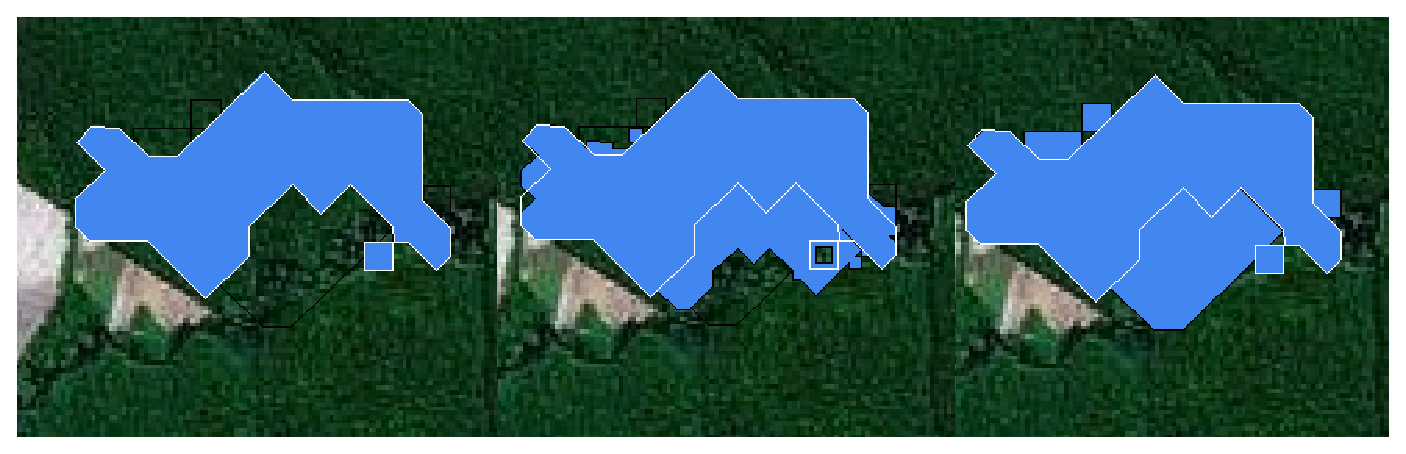
\includegraphics[width=0.9 \textwidth]{DeterUnit.eps}}
\subfigure{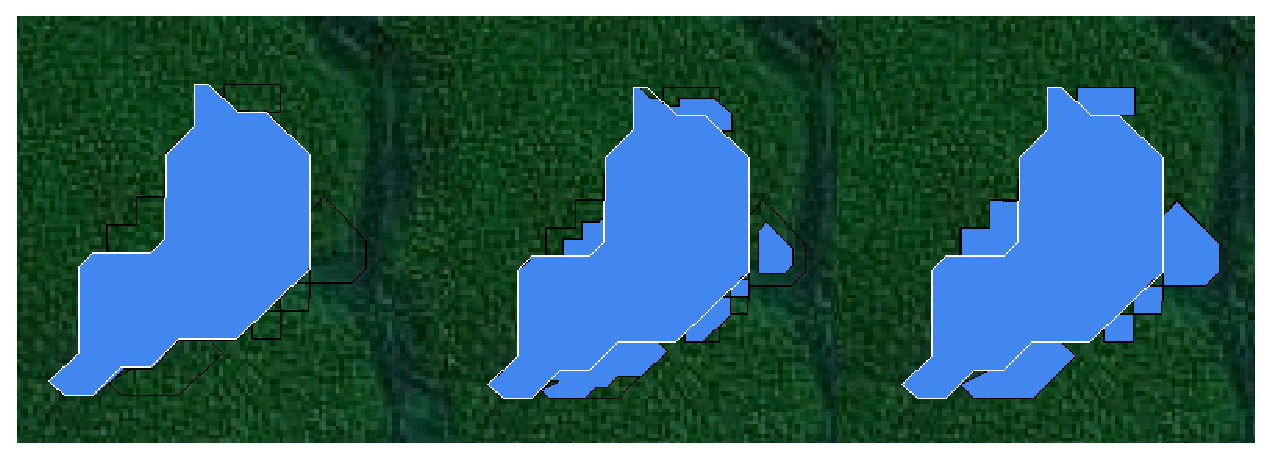
\includegraphics[width=0.9 \textwidth]{DeterUnit2.eps}}		\subfigure{\includegraphics[width=0.9 \textwidth]{DeterUnit3.eps}}		
	\caption[Region--Unit aus Deter--Daten]{Je drei Momentaufnahmen dreier Region--Units, die aus den Deter--Daten gewonnen wurden.\\\textit{\begin{tabular}{ll}
Quelle: &Luftbild, Google Maps;\\
&DETER-Daten dargestellt mit SECONDO
\end{tabular}}}
	\label{fig:RegionUnitDeter}
\end{figure}


%\section{Die Konstruktion der Moving-Regions}
